\titledquestion{Multiple Choices}

Each question has \textbf{one or more} correct answer(s). Select all the correct answer(s). For each question, you will get 0 points if you select one or more wrong answers, but you will get 1 point if you select a non-empty subset of the correct answers.

Write your answers in the following table.

%%%%%%%%%%%%%%%%%%%%%%%%%%%%%%%%%%%%%%%%%%%%%%%%%%%%%%%%%%%%%%%%%%%%%%%%%%%
% Note: The `LaTeX' way to answer a multiple-choice question is to replace `\choice'
% with `\CorrectChoice', as what you did in the first question. However, there are still
% many students who would like to handwrite their homework. To make TA's work easier,
% you have to fill in your selected choices in the table below, no matter whether you use
% LaTeX or not.
%%%%%%%%%%%%%%%%%%%%%%%%%%%%%%%%%%%%%%%%%%%%%%%%%%%%%%%%%%%%%%%%%%%%%%%%%%%

\begin{table}[htbp]
    \centering
    \begin{tabular}{|p{2cm}|p{2cm}|p{2cm}|p{2cm}|}
        \hline
        (a) & (b) & (c) & (d) \\
        \hline
        %%%%%%%%%%%%%%%%%%%%%%%%%%%%
        % YOUR ANSWER HERE.
            &  &  &    \\
        %%%%%%%%%%%%%%%%%%%%%%%%%%%%
        \hline
        (e) & (f) & (g) & (h) \\
        \hline
        %%%%%%%%%%%%%%%%%%%%%%%%%%%%
        % YOUR ANSWER HERE.
            &  &  &   \\
        %%%%%%%%%%%%%%%%%%%%%%%%%%%%
        \hline
    \end{tabular}
\end{table}


\begin{parts}

\part[2] Which of the following statements is/are \textbf{TRUE}?
\begin{choices}
\choice Dijkstra algorithm can find the shortest path in any DAG.
\choice If we use the Dijkstra algorithm, whether the graph is directed or undirected does not matter.
\choice At each iteration of the Dijkstra algorithm, we pop the vertex with the shortest current distance to the start vertex, while in the Prim algorithm, we pop the vertex with the shortest distance to the current minimum spanning tree.
\choice In directed graph $G = (V, E)$, if $(s, v_1, v_2, v_3, v_4, t)$, where $s, v_i, t \in V$ , is the shortest path from $s$ to $t$ in $G$, then $(v_1, v_2, v_3, v_4)$ must be the shortest path from $v_1$ to $v_4$ in $G$.
\end{choices}


\part[2] Which of the following statements is/are \textbf{TRUE}?
\begin{choices}
\choice Bellman-Ford algorithm can find the shortest path for negative-weighted directed graphs, while the Dijkstra algorithm may fail.
\choice The run time of the Bellman-Ford algorithm is $O(|V||E|)$, which is more time-consuming than the Dijkstra algorithm with heap implementation.
\choice Topological sort can be extended to determine whether a graph has a cycle while the Bellman-Ford algorithm can be extended to determine whether a graph has a negative cycle.
\choice Topological sort can find the critical path in a DAG while the Bellman-Ford algorithm can find the single-source shortest path in a DAG.
\end{choices}


\part[2] Given an undirected graph $G = (V, E)$ with its minimum spanning tree $T \subset  E$, which of the following statements is/are \textbf{TRUE}?
\begin{choices}
\choice  Both the Prim algorithm and the Dijkstra algorithm can run in time complexity $O(|E| \log |V |)$.
\choice After negating all weights of edge in $G$ and getting the new graph $G'$, apply the original Prim algorithm on $G'$ will find the Maximum Spanning Tree of $G$. Similarly, applying the Dijkstra algorithm will find the longest distance.
\choice We prefer Dijkstra's algorithm with binary heap implementation to the naive adjacency matrix implementation in a dense graph where $|E| = \Theta(|V|^2)$
\choice  For any vertex $v$ in $G$ such that the shortest paths from $v$ to all other vertices in $V$ are the same as the shortest paths only using edges in $T$.
\end{choices}


\part[2] Which of the following statements about shortest path algorithms is/are \textbf{TRUE}?
\begin{choices}
\choice If we modify the outer loop of the Bellman-Ford algorithm to execute $|V|$ iterations instead of $|V|-1$ iterations, the algorithm can still find the shortest path on a directed graph with negative-weight edges but no negative cycles.
\choice We can modify the Bellman-Ford algorithm to find the longest path in a directed graph with positive-weight edges but no positive cycles.
\choice We can modify the Floyd-Warshall algorithm to detect whether there exists a negative cycle or not in a directed graph.
\choice If we modify the out-most loop of the Floyd-Warshall algorithm to execute $|V|-1$ iterations instead of $|V|$ iterations, the algorithm can still find all pairs of shortest paths on a directed graph with negative-weight edges but no negative cycles.
\end{choices}


\part[2] Which of the following is/are \textbf{TRUE}?
\begin{choices}
    \choice The A* graph search algorithm with a consistent heuristic will always return an optimal solution if it exists.
    \choice The A* graph search algorithm with an admissible heuristic will always return an optimal solution if it exists.
    \choice The A* tree search algorithm with a consistent heuristic will always return an optimal solution if it exists.
    \choice The A* tree search algorithm with an admissible heuristic will always return an optimal solution if it exists.
\end{choices}


\part[2] Which of the following is/are \textbf{TRUE}?
\begin{choices}
    \choice Dijkstra algorithm can be viewed as a special case of the A* Graph Search algorithm where the heuristic function from any vertex $u$ to the terminal $z$ is $h(u, z)=0$.
    \choice Floyd-Warshall algorithm can always give the correct shortest distance between any two vertices in directed graphs with negative weights.
    \choice In A* graph search algorithm with a consistent heuristic function, if vertex $u$ is marked visited before $v$, then $d(u)+h(u)\leq d(v)+h(v)$, where $d(u)$ is the distance from the start vertex to $u$.
    \choice Bellman-Ford algorithm can work correctly on any graphs with negative edges.
\end{choices}


\part[2] We run the Floyd-Warshall algorithm on a simple graph without negative cycles with $3n$ vertices $v_1, \ldots, v_{n}, \ldots, v_{2n}, \ldots,  v_{3n}$. Suppose all three loops $(k, i, j)$ are iterated from $1$ to $3n$. After running at least how many iterations of the out-most loop $k$, it is ensured to find the shortest path between $v_{2n}$ and $v_{3n}$?
\begin{choices}
\choice $2n-1$
\choice $2n$
\choice $3n-1$
\choice $3n$
\end{choices}


\part[2] To solve the $N$ Puzzle problems with the A* search, which of the following heuristics is/are admissible?
\begin{figure}[H]
    \centering
    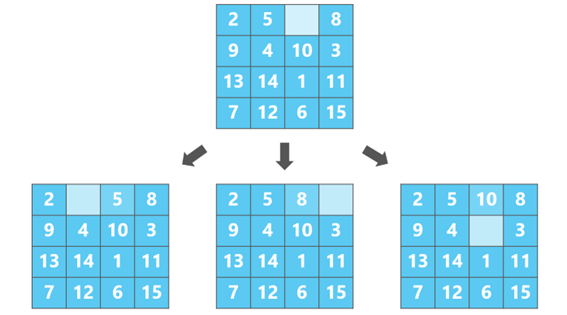
\includegraphics[width=0.5\linewidth]{figure/puzzle.png}
    \caption{A kind of $15$ puzzle}
\end{figure}

\begin{choices}
\choice $h =$ if the state is the goal state, it is $1$; otherwise, it is $0$
\choice $h =$ number of misplaced tiles
\choice $h =$ the sum of the minimum number of moves required to put each tile in its correct location
\choice $h =$ actual minimum number of moves required to put all tiles in their correct location.
\end{choices}

\end{parts}